The first figure groups the card labels by actual self-pairs and cross-pairs. The undisclosed condition supplies a separate baseline within each actual group.

\begin{figure*}[t]
\centering
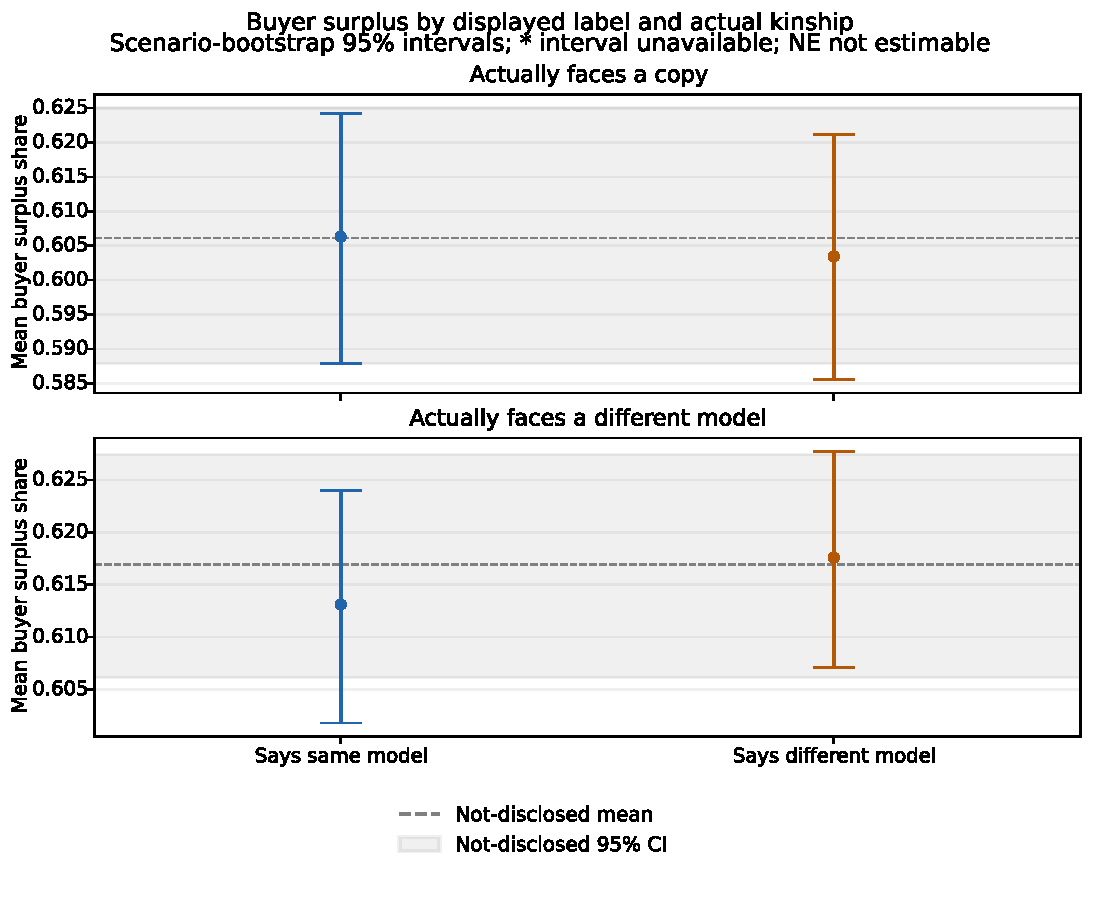
\includegraphics[width=\textwidth]{appendix/figures/study2-main_label_by_actual_kinship.pdf}
\caption{Study 2 displayed labels and actual kinship: means and scenario-bootstrap intervals. The shared baseline legend is moved below the panels for legibility; the dashed grey line and shading give the undisclosed mean and interval in each panel.}
\label{fig:appendix-study2-main_label_by_actual_kinship}
\end{figure*}

The next figure shows deal rates and surplus shares among completed deals. The latter conditions on agreement and must be read as a deal-only outcome.

\begin{figure*}[t]
\centering
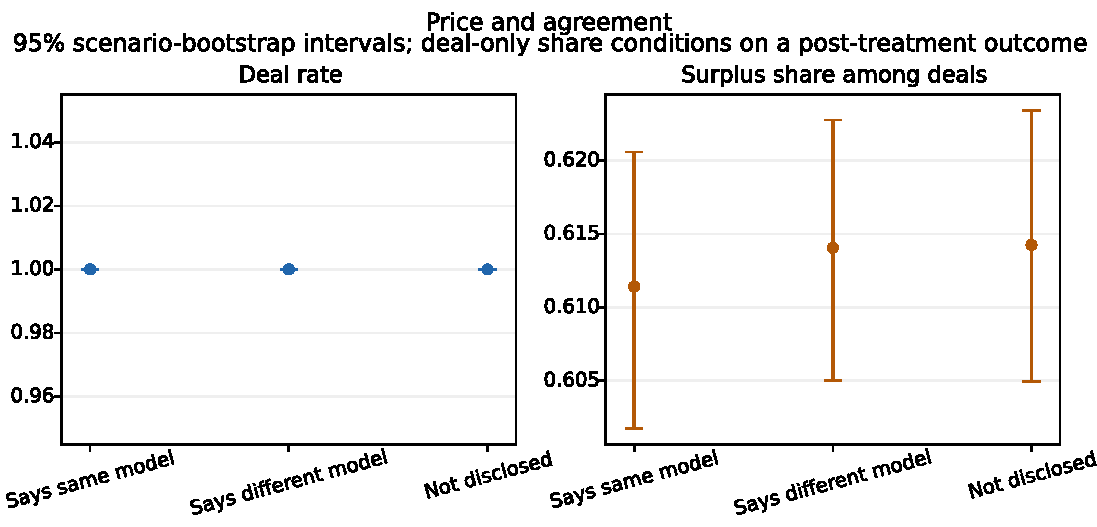
\includegraphics[width=\textwidth]{appendix/figures/study2-deal_rate_and_within_deal_share.pdf}
\caption{Study 2 deal rate and share among deals, grouped by what the card says.}
\label{fig:appendix-study2-deal_rate_and_within_deal_share}
\end{figure*}

The buyer-specific plot shows each registered P2 contrast with its scenario-bootstrap interval. These are secondary comparisons.

\begin{figure*}[t]
\centering
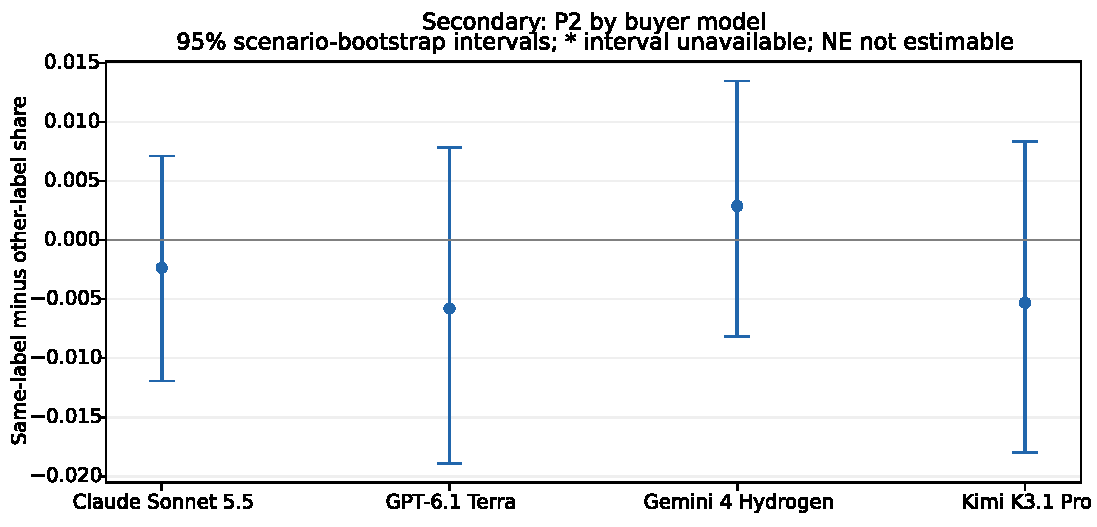
\includegraphics[width=\textwidth]{appendix/figures/study2-appendix_buyer_p2.pdf}
\caption{Study 2 P2 by buyer model: same minus other, in buyer-share units.}
\label{fig:appendix-study2-appendix_buyer_p2}
\end{figure*}

The final plot displays the distribution of buyer shares by original disclosure condition. It includes impasses according to the registered zero rule.

\begin{figure*}[t]
\centering
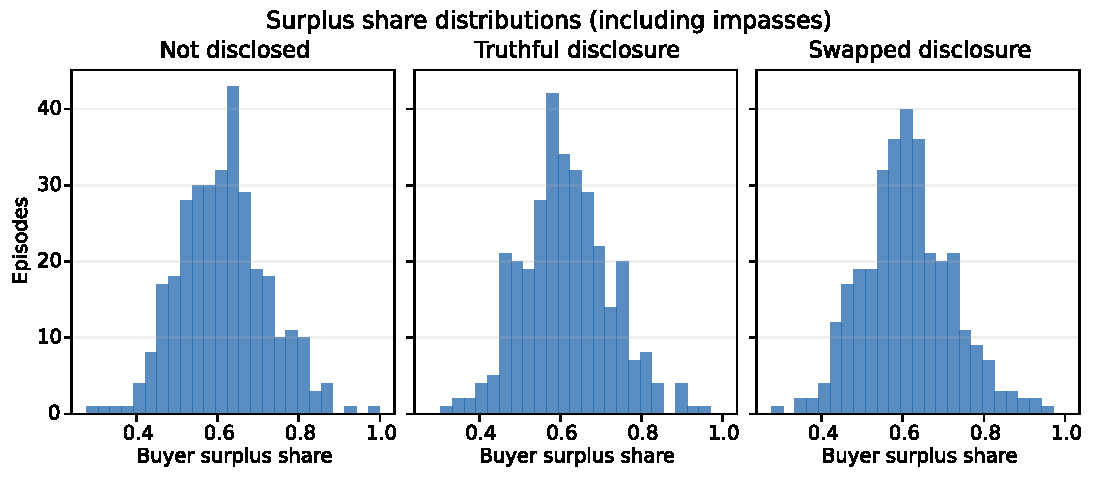
\includegraphics[width=\textwidth]{appendix/figures/study2-appendix_share_distributions.pdf}
\caption{Study 2 surplus-share distributions by original disclosure condition.}
\label{fig:appendix-study2-appendix_share_distributions}
\end{figure*}

